\documentclass[11pt]{article}

\usepackage[utf8]{inputenc}
\usepackage[T1]{fontenc}
\usepackage[margin=1in]{geometry}
\usepackage{amsmath,amssymb,amsthm,mathtools}
\usepackage{booktabs}
\usepackage{enumitem}
\usepackage{xcolor}
\usepackage{pgfplots}
\pgfplotsset{compat=1.18}
\usepackage[colorlinks=true,linkcolor=black,citecolor=black,urlcolor=blue]{hyperref}

\theoremstyle{plain}
\newtheorem{theorem}{Theorem}
\newtheorem{proposition}{Proposition}
\newtheorem{lemma}{Lemma}
\newtheorem{corollary}{Corollary}
\theoremstyle{definition}
\newtheorem{definition}{Definition}
\newtheorem{axiom}{Axiom}
\theoremstyle{remark}
\newtheorem{remark}{Remark}

\newcommand{\V}{\mathrm{V}}
\newcommand{\R}{\mathrm{R}}
\newcommand{\confidence}{\operatorname{confidence}}
\newcommand{\Supply}{\operatorname{Supply}}
\newcommand{\VerifiedValue}{\operatorname{VerifiedValue}}
\newcommand{\ExtRev}{\mathrm{ExtRev}}
\newcommand{\Turnover}{\operatorname{Turnover}}

\title{\textbf{Kredo}: A Contribution-Based Mutual-Credit Economy\\
with Soulbound Reputation and Compensatory Emission}

\author{Fedor Chishchin\\
\small Independent Researcher\\
\small \texttt{fedorstartup@gmail.com}}

\date{\today}

\begin{document}
\maketitle

\begin{abstract}
We present \emph{Kredo}, an economic mechanism designed to reward the creation of value rather than the position of ownership. The design is derived top-down: five philosophical axioms are formalized as seven state invariants, and every transition function is required to preserve them. The economy uses two assets: a transferable contribution token $\V$ (working money and a claim on the club's external profit) and a non-transferable ``soulbound'' reputation token $\R$. Credit is issued at the moment of a confirmed transaction and accompanied by a \emph{compensatory emission}---a deferred, escrowed ``dividend to all'' whose magnitude is governed by a dynamic coefficient $\varepsilon$ that shrinks as the observed default rate grows. We prove that this coefficient keeps the money supply bounded relative to verified value even under nonzero defaults (Theorem~\ref{thm:stability}), and that operations against the liquidity fund are price-neutral (Theorem~\ref{thm:neutrality}), so the price cannot be moved by fund operations. Governance uses quadratic ($\sqrt{\R}$) voting under a dual reputation-and-stake quorum, which, together with the soulbound property of $\R$, forces any would-be captor to win a majority of verified, active reputation and a majority of circulating stake simultaneously. We derive a minimal external-revenue-growth \emph{survival condition} for a non-declining price, show that the discounted-withdrawal rule leaves the fund positive at every partial level of exit, and prove a stake threshold of order $\bar N/a$ beyond which even the optimal adaptive wash-trading fraud is unprofitable. A deterministic agent-based simulator implementing the full mechanism is exercised across $315$ stability runs---Monte~Carlo, a $192$-point parameter sweep, and combined-attack stress tests---none of which produced an economic collapse, while a separate regime analysis reproduces the predicted price trajectories. All code, derivations, and results are released openly.
\end{abstract}

\noindent\textbf{Keywords:} mutual credit; complementary currency; mechanism design; token economics; quadratic voting; Sybil resistance; agent-based simulation.

\smallskip
\noindent\textbf{JEL codes:} D47; D71; E42; C63.

\section{Introduction}

Two widely deployed classes of economic organization each embed a structural unfairness. In \emph{rent-based capitalism}, the holder of capital earns without contributing: value is extracted from a position of ownership rather than created, and the producer of value and the recipient of profit are frequently distinct agents. In \emph{egalitarian cooperatives and communes}, all members are treated equally, but the absence of a growth-and-reward mechanism yields the classical free-rider problem: contribution is not differentially rewarded, active members bear disproportionate cost, and the system stagnates.

This paper studies a mechanism, \emph{Kredo}, intended as a third option: reward proportional to the creation of value, in which active members earn more than passive ones yet no member is left with nothing, and in which the system defends itself against inflation, panic, and fraud without discretionary intervention.

Our contributions are as follows.
\begin{enumerate}[leftmargin=*,itemsep=2pt]
    \item A top-down design method: five axioms (Section~\ref{sec:axioms}) are formalized as seven invariants that every transition function must preserve (Section~\ref{sec:invariants}), yielding a specification in which the intended ethics are machine-checkable properties.
    \item A compensatory-emission mechanism with a dynamic coefficient $\varepsilon$, and a proof that it bounds supply relative to verified value under nonzero defaults (Theorem~\ref{thm:stability}).
    \item A pricing rule tied strictly to fundamentals, with a proof that fund operations are price-neutral (Theorem~\ref{thm:neutrality}) and that the discounted-withdrawal rule cannot exhaust the fund under a run (Theorem~\ref{thm:norun}).
    \item A governance design combining $\sqrt{\R}$ voting with a dual quorum and a soulbound reputation token---capital buys no reputation votes, and Sybil identities are contained by screening cost and the stake quorum rather than by the vote rule (Proposition~\ref{prop:sybil})---and a characterization of exactly when wash-trading fraud, including the optimal adaptive strategy, is unprofitable (Theorems~\ref{thm:fraud} and~\ref{thm:deter}).
    \item A minimal external-revenue survival condition with the long-run price limit (Propositions~\ref{prop:survival} and~\ref{prop:longrun}), a consolidated set of deployment conditions (Section~\ref{sec:guidance}), and an empirical validation over $315$ simulated runs.
\end{enumerate}

All artifacts---the mechanism, its derivations, the simulator, the experiment protocols, and the raw results---are publicly available.\footnote{\url{https://github.com/fedorello/kredo-model}}

\section{Related work}\label{sec:related}

The idea that money should not accrue rent to idle holders traces to Gesell's proposal of a carrying cost on currency \cite{gesell1916}. Mutual-credit systems, in which the money supply is created endogenously by bilateral trade and nets to zero, have a long practical history \cite{greco2009}; empirical work on the Swiss WIR/\emph{Wirtschaftsring} documents their counter-cyclical, macro-stabilizing behavior \cite{stodder2009}. Contemporary blockchain-based complementary currencies such as Circles~UBI \cite{circles2020} and GoodDollar \cite{gooddollar2021} distribute newly issued units broadly; Kredo's ``dividend to all'' is a deferred, contribution-weighted, default-conditioned variant of this idea. Trustless issuance and the avoidance of pre-mine follow the design ethos of permissionless value systems \cite{nakamoto2008}. Our governance draws on quadratic voting \cite{lalley2018} and quadratic funding \cite{buterin2019}, whose square-root weighting limits plutocratic dominance; the soulbound (non-transferable) treatment of reputation is what makes the quadratic weighting robust to vote-buying. Resistance to Sybil attacks is analyzed in the tradition of Douceur \cite{douceur2002}. Finally, we evaluate the mechanism with agent-based simulation \cite{bonabeau2002}, the standard tool for studying emergent behavior of many interacting agents when closed-form analysis is intractable. Table~\ref{tab:related} positions Kredo's design choices against the most closely related systems.

\begin{table}[h]
\centering
\small
\begin{tabular}{@{}lllll@{}}
\toprule
System & Money creation & Backing / exit & Sybil defense & Governance\\
\midrule
WIR \cite{stodder2009} & mutual credit & none (no redemption) & bank vetting & cooperative bank\\
Time banks \cite{greco2009} & hour credits & none & community vetting & informal\\
Circles~UBI \cite{circles2020} & equal per-person UBI & none & web of trust & community\\
GoodDollar \cite{gooddollar2021} & daily UBI & crypto reserve & identity check & foundation/DAO\\
\addlinespace
Kredo & gated credit $+$ & USDC fund, formula & KYC-light $+$ soulbound & $\sqrt{\R}$, dual\\
      & escrowed dividend & price, discount queue & $\R$, $\sqrt{\R}$ votes & quorum\\
\bottomrule
\end{tabular}
\caption{Kredo against related complementary-currency systems (coarse characterization).}
\label{tab:related}
\end{table}

\section{The model}

\subsection{Axioms}\label{sec:axioms}

\begin{axiom}[Value is created, not extracted]\label{ax:create}
Reward must correspond to the creation of value, not to a position of ownership.
\end{axiom}
\begin{axiom}[Value is subjective but consensual]\label{ax:price}
A fair price is the one two parties agree upon voluntarily under the availability of alternatives.
\end{axiom}
\begin{axiom}[Symmetry of gain and loss]\label{ax:symmetry}
All participants are structurally bound to the fate of the system; no class is shielded from the risks of the others.
\end{axiom}
\begin{axiom}[No privileged knowledge]\label{ax:transparency}
All rules, balances, and decisions are transparent.
\end{axiom}
\begin{axiom}[Power from contribution]\label{ax:power}
Influence over the rules follows from demonstrated useful participation, not from accumulated capital.
\end{axiom}

\subsection{State}

\begin{definition}[System state]
At discrete time $t$ the state is the tuple
\[
S_t = (M_t,\ b_t,\ r_t,\ d_t,\ F_t,\ E_t,\ G_t,\ H_t),
\]
where $M_t$ is the finite set of members; $b_t: M_t \to \mathbb{R}$ the $\V$-balance (which may be negative up to a credit limit); $r_t: M_t \to \mathbb{R}_{\ge 0}$ the reputation; $d_t: M_t \to \mathbb{R}_{\ge 0}$ accumulated debt; $F_t \in \mathbb{R}_{\ge 0}$ the liquidity fund (in an external stable asset, USDC); $E_t \in \mathbb{R}_{\ge 0}$ the distribution escrow; $G_t \in \mathbb{R}_{\ge 0}$ the genesis pool; and $H_t$ the append-only transaction history.
\end{definition}

\subsection{Invariants}\label{sec:invariants}

The seven invariants below formalize Axioms~\ref{ax:create}--\ref{ax:power}. Let $N_{\mathrm{credit}}(\tau)$ be the newly issued (credit) portion of transaction $\tau$, admitted only when its trust score $\confidence(\tau)\in[0,1]$ (Section~\ref{sec:confidence}) clears the gate of (I2); write $C(\tau)=N_{\mathrm{credit}}(\tau)$ for this \emph{confirmed contribution}.

Because Kredo is a mutual-credit system, a loan's contribution to circulating supply depends on its state: while \emph{open}, its principal circulates and its compensation waits in escrow; \emph{repayment annihilates the principal} (the debtor's incoming units cancel the debt and leave circulation) and releases the escrow; a \emph{good-faith default} retains the circulating principal---backed by the work actually delivered---but burns the escrow; \emph{remediated fraud} burns both. Accordingly, write
\[
\Supply(t) = \sum_{m} \max\bigl(0,b_t(m)\bigr) + E_t + G_t, \qquad
\VerifiedValue(t) = \sum_{\tau \in H_t} v_t(\tau) \;+\; \Gamma_t \;+\; \mathrm{Invested}_t \;-\; \mathrm{Burned}(t),
\]
with the loan-state contribution
\[
v_t(\tau)=\bigl(1+\varepsilon(\tau)\bigr)C(\tau),\quad \varepsilon(\tau)\,C(\tau),\quad C(\tau),\quad 0
\]
for open, repaid, good-faith-defaulted, and fraud-remediated loans respectively, where $\varepsilon(\tau)$ is the compensation coefficient of \eqref{eq:epsilon} (defined in Section~\ref{sec:emission}) fixed at the time of $\tau$; $\Gamma_t$ is the cumulative genesis issuance (minted into the pool, itself funded by realized external revenue and fines, Section~\ref{sec:emission}); $\mathrm{Invested}_t$ is the cumulative $\V$ issued to investors against USDC at the fundamental price of (I5), fully backed by the fund at issuance; and $\mathrm{Burned}(t)$ counts \emph{only} conversions and penalties levied outside the loan lifecycle---escrow burned at default and principal burned at fraud remediation are already reflected in $v_t$ and are not double-counted. With this bookkeeping $\Supply$ and $\VerifiedValue$ coincide up to the lag between fraud and its detection. It matches the reference implementation's (I3) checker, which likewise tracks contribution by loan state; that checker's stricter variant additionally weights $C(\tau)$ by $\confidence(\tau)$---a second, small drift source, since most transactions clear the auto-check at $\confidence=1$.

\begin{description}[leftmargin=*,itemsep=3pt]
    \item[(I1) Conservation on transfers.] For any pure transfer, $\sum_{m} b_{t}(m) = \sum_{m} b_{t+1}(m)$.
    \item[(I2) Gated emission.] Unbacked $\V$ is minted only within the confirmation protocol and only if $\confidence(\tau) \ge \theta_{\min}$; the only other issuance channels are fully backed---\textsc{Invest} at the fundamental price of (I5) and genesis issuance funded by realized revenue and fines.
    \item[(I3) Supply tracks value.] $\bigl|\Supply(t) - \VerifiedValue(t)\bigr| \le \epsilon_{\mathrm{tol}}\,\Supply(t)$, with $\epsilon_{\mathrm{tol}} = 0.05$ absorbing detection lag.
    \item[(I4) Credit limit.] $b_t(m) \ge -L\bigl(r_t(m)\bigr)$ for all $m,t$.
    \item[(I5) Fundamental price.] $P_t = \bigl(F_t + \mu\,\ExtRev_t\bigr)/\Supply(t)$ is always computed, never assigned.
    \item[(I6) Soulbound reputation.] No transfer map for $\R$ exists; $\R$ is only minted (for merit) and burned (for violations).
    \item[(I7) Universal rules.] Every function depends only on observable state $(b,r,d)$, not on member identity.
\end{description}

The admissible transition functions are \textsc{Join}, \textsc{Leave}, \textsc{Transact}, \textsc{Repay}, \textsc{Default}, \textsc{Convert}, \textsc{Invest}, together with derived periodic operations; each is required to preserve (I1)--(I7).

\subsection{Notation and default parameters}

Table~\ref{tab:notation} collects the recurring symbols; every default is governable within the bounds of Section~\ref{sec:guidance}.

\begin{table}[h]
\centering
\small
\begin{tabular}{@{}lll@{}}
\toprule
Symbol & Meaning & Default\\
\midrule
$b,r,d$ & member balance, reputation, debt & ---\\
$F_t,\ E_t,\ G_t$ & liquidity fund (USDC), escrow, genesis pool & ---\\
$S=\Supply$ & positive balances $+$ escrow $+$ genesis & ---\\
$P_t$ & price $(F+\mu\,\ExtRev)/S$ & $\mu=12$\\
$L(r)$ & credit limit $L_0(1+\alpha\ln(1+r))$ & $L_0=100$, $\alpha=0.5$\\
$\confidence(\tau)$ & trust score; emission gate & $\theta_{\min}=0.6$\\
$a$ & stochastic audit rate per transaction & $0.03$\\
$\varepsilon(t)$ & compensation coefficient \eqref{eq:epsilon} & $K^*{=}1.5$, $\delta^*{=}0.05$, $\kappa{=}2$, $\varepsilon_{\max}{=}0.95$\\
$\delta_t$ & observed default rate ($90$-day window) & ---\\
$\rho_t,\ \rho^*$ & fund coverage $F/(PS)$; discount threshold & $\rho^*=0.3$\\
$\tau_{\mathrm{lock}}$ & conversion lock-up for new balances & $60$ days\\
$g_0,\ \xi$ & genesis grant; distribution smoothing & $g_0\le100~\V$, $\xi=1$\\
$\theta$ & dual-quorum threshold & $0.5$ ($0.66$ constitutional)\\
$\bar N$ & mean transaction size & $50~\V$ (illustrative)\\
$\beta,\ c,\ p$ & fraud hazard $\ln(1/(1-a))/\bar N$; lock-up survival $(1-p)^{\tau_{\mathrm{lock}}}$; $p$ per-period detection & ---\\
$\Lambda$ & forfeitable stake per fraud cluster & $300~\V$ (illustrative); threshold $\Lambda\ge\bar N/a$\\
\bottomrule
\end{tabular}
\caption{Notation and default parameters.}
\label{tab:notation}
\end{table}

The reputation coefficients $\beta_{1\ldots4}$ (Section~6), the transaction category $c$ of $\tau$ (Section~\ref{sec:confidence}), and the asset growth rate $g$ of Proposition~\ref{prop:longrun} are local symbols, distinct from the fraud parameters $\beta$, $c$ and the profit bound $g(W)$.

\section{Credit and confidence}\label{sec:confidence}

\subsection{Credit limit}

\begin{equation}\label{eq:limit}
L(r) = L_0\bigl(1 + \alpha \ln(1+r)\bigr), \qquad L_0 = 100~\V,\ \ \alpha = 0.5.
\end{equation}
The logarithm bounds exposure: a member with $r = 10^4$ borrows at most $\approx 561~\V$, only ${\approx}5.6\times$ a newcomer's limit (Table~\ref{tab:limit}). No single agent can therefore threaten solvency by defaulting.

\begin{table}[h]
\centering
\begin{tabular}{lrrrrrr}
\toprule
$r$ & $0$ & $1$ & $10$ & $100$ & $1000$ & $10000$\\
\midrule
$L(r)$ & $100$ & $135$ & $220$ & $331$ & $445$ & $561$\\
\bottomrule
\end{tabular}
\caption{Credit limit \eqref{eq:limit} as a function of reputation, rounded to the nearest integer.}
\label{tab:limit}
\end{table}

\subsection{Confidence}

Axiom~\ref{ax:price} forbids the mechanism from setting prices; instead it estimates how much a declared price can be trusted before minting against it. For a transaction $\tau=(A,B,N,c)$ with provider $A$, receiver $B$, declared value $N$, and category $c$,
\begin{equation}
\confidence(\tau) = w_a s_a(\tau) + w_r s_r(\tau) + w_x s_x(\tau), \qquad w_a+w_r+w_x=1 .
\end{equation}
The \emph{auto-score} compares $N$ to the category's recent price distribution. With sample mean $\mu_c$ and standard deviation $\sigma_c$ over a $90$-day window and $z = (N-\mu_c)/\sigma_c$,
\begin{equation}\label{eq:autoscore}
s_a(\tau) = \begin{cases} 1, & |z| \le 1,\\[3pt] \exp\!\left(-\dfrac{(|z|-1)^2}{2}\right), & |z| > 1. \end{cases}
\end{equation}
Thus $s_a = 0.61,\,0.14,\,0.01$ at $z = 2,3,4$; for a degenerate or new category ($\sigma_c=0$), review is mandatory. The \emph{review-score} $s_r$ is the median vote of randomly drawn reviewers (robust to outliers), and the \emph{audit-score} $s_x$ is $1$ unless a stochastic audit finds a violation. Review is triggered when $|z|>1$, when $N$ exceeds the auto-approval limit $N_{\mathrm{auto}} = 50\sqrt{r_A r_B + 1}$, when a party is under monitoring, or when the $3\%$ random audit selects $\tau$. Emission proceeds only when $\confidence(\tau) \ge \theta_{\min} = 0.6$, per invariant (I2).

\subsection{Market health and anti-concentration}

Axiom~\ref{ax:price} locates dishonesty not in a ``wrong'' price but in the absence of alternatives; accordingly the mechanism monitors structural market health rather than individual prices. For each service category it tracks a Herfindahl--Hirschman concentration index, the bilateral concentration of a member's counterparties, and short-cycle reciprocity (a signature of wash trading). When a category or cluster is flagged, the response is graduated and non-price: reduced credit limits for the implicated cluster, an elevated audit rate, suspension of compensatory emission on suspect transactions, and, in the limit, escalation to a community vote. The mechanism thus defends the \emph{conditions} of honest exchange---transparency and the availability of alternatives---rather than dictating terms.

\section{Emission and the compensation coefficient}\label{sec:emission}

\subsection{Mechanics}

In \textsc{Transact}, the credit portion is $N_{\mathrm{credit}} = \max\bigl(0,\ N - \max(0,b_B)\bigr)$; the provider is credited $N$, and $B$'s balance decreases by $N$, opening a debt of $N_{\mathrm{credit}}$ when $b_B < N$ (a pure transfer when $N_{\mathrm{credit}}=0$). Simultaneously a \emph{compensatory emission} enters escrow,
\begin{equation}\label{eq:comp}
\Delta E = \varepsilon(t)\, N_{\mathrm{credit}} .
\end{equation}
The escrow is released pro rata upon repayment and \emph{burned} upon default. Released amounts are distributed across members in proportion to active turnover, where
\[
\Turnover(m,t) = \sum_{\tau:\ t-\tau<90d,\ m\in\tau} N(\tau)\,\confidence(\tau),
\]
via
\begin{equation}
\mathrm{Share}(m,t) = \frac{\Turnover(m,t) + \xi}{\sum_{m'}\Turnover(m',t) + n_t\,\xi}, \qquad \xi = 1,\ \ n_t=|M_t|,
\end{equation}
so the ``dividend to all'' rewards active contribution rather than idle holdings. The coefficient is dynamic in the observed default rate $\delta_t$:
\begin{equation}\label{eq:epsilon}
\varepsilon(t) = \max\!\Bigl(0,\ \min\bigl(\varepsilon_{\max},\ K^* - 1 - \kappa\,(\delta_t - \delta^*)\bigr)\Bigr),
\end{equation}
with defaults $K^* = 1.5$, $\delta^* = 0.05$, $\kappa = 2$, $\varepsilon_{\max}=0.95$. Hence $\varepsilon$ ranges from $0.60$ at $\delta=0$ down to $0$ at $\delta = 0.30$.

\subsection{Stability under defaults}

\begin{theorem}[Bounded supply under defaults]\label{thm:stability}
Consider a stationary credit regime---abstracting from genesis and investor issuance, both of which are fully backed at issuance---in which every loan resolves as repaid (fraction $1-\delta$), defaulted in good faith (fraction $\delta_g$), or detected-and-remediated fraud (fraction $\delta_f$), with $\delta=\delta_g+\delta_f\in[0,1)$ and $\varepsilon$ given by \eqref{eq:epsilon}. Assume $K^*\ge\max(1,\varepsilon_{\max})$ (true of the defaults, where $\varepsilon_{\max}=0.95<1\le K^*$). Let $C_{\mathrm{tot}}=\sum_\tau C(\tau)$ and let $P_{\mathrm{net}}=(1-\delta_f)\,C_{\mathrm{tot}}$ be the contribution backed by delivered work. Then
\[
\frac{\Supply}{P_{\mathrm{net}}} \;=\; \frac{(1-\delta)\,\varepsilon+\delta_g}{1-\delta_f}\;\le\;\max(1,\varepsilon_{\max})\;\le\;K^*.
\]
\end{theorem}

\begin{proof}
By the loan-state bookkeeping of Section~\ref{sec:invariants}, a repaid unit of contribution leaves $\varepsilon$ in circulation (principal annihilated by repayment, escrow released), a good-faith default leaves $1$ (principal retained, escrow burned), and remediated fraud leaves $0$. Hence $\Supply = C_{\mathrm{tot}}\bigl[(1-\delta)\varepsilon+\delta_g\bigr]$, giving the stated ratio. Since $(1-\delta)+\delta_g = 1-\delta_f$, the numerator is a sub-convex combination: $(1-\delta)\varepsilon+\delta_g \le \max(1,\varepsilon)\bigl[(1-\delta)+\delta_g\bigr] = \max(1,\varepsilon)(1-\delta_f)$, so the ratio is at most $\max(1,\varepsilon)$. Finally $\varepsilon\le\varepsilon_{\max}$ by \eqref{eq:epsilon}, and $\max(1,\varepsilon_{\max})\le K^*$ by hypothesis.
\end{proof}

\begin{remark}
Theorem~\ref{thm:stability} is the inflation brake, and it holds for \emph{any} mix of defaults: repayment annihilates principal (only the $\varepsilon$-dividend survives), a good-faith default leaves principal that is backed by delivered work, and the only unbacked issuance---fraud---is burned on detection. As realized defaults rise, $\varepsilon$ falls automatically by \eqref{eq:epsilon}, and at $\delta=0.30$ compensation is disabled entirely (strict conservation). The one channel the theorem does not cover, fraud that is never detected, is quantified in Proposition~\ref{prop:genstab}.
\end{remark}

The genesis grant to a joining member, $g_0 = \min\bigl(100,\ G_t/\mathbb{E}[\text{new members}]\bigr)$, is likewise self-limiting: it contracts if growth outpaces the pool's inflow, so no subsidy is created \emph{ex nihilo}.

\subsection{Debt resolution and reactivation}

Overdue debt triggers graduated sanctions rather than exclusion: at $30$, $60$, and $90$ days the debtor faces escalating reputation decay and, ultimately, a freeze (balance and reputation reset, escrow burned) instead of expulsion. A frozen member may reactivate by repaying the outstanding debt and completing a probationary period restricted to small transactions. This regenerative treatment follows from Axiom~\ref{ax:create}: the objective is to restore productive participation, not to punish.

\section{Reputation and governance}

Reputation accrues through concave (activity) and linear (quality) terms and burns for failures:
\begin{align}
\Delta \R &= \beta_1 \ln(1 + n_{\mathrm{tx}}) + \beta_2\, a_{\mathrm{audit}} + \beta_3 \ln(1 + \text{tenure}/30) + \beta_4\, n_{\mathrm{disputes}},\\
\Delta \R^{-} &= \gamma_1 f_{\mathrm{review}} + \gamma_2 f_{\mathrm{dispute}} + \gamma_3\, \mathrm{DefaultPenalty} + \gamma_4\, \mathrm{Fraud},
\end{align}
where $n_{\mathrm{tx}}$ counts confirmed transactions, $a_{\mathrm{audit}}$ correct audit decisions, $n_{\mathrm{disputes}}$ disputes resolved as arbiter, and $f_{\mathrm{review}}, f_{\mathrm{dispute}}$ failed reviews and lost disputes; the coefficients $\beta_{1\ldots4},\gamma_{1\ldots4}$ are governable, with $\gamma_4 = 100$: proven fraud erases years of reputation. Concavity in bulk actions prevents reputation farming by volume.

Voting power is $\sqrt{\R(m)}$. Strategic decisions require a \emph{dual quorum}: a reputation quorum $\sum_{\text{voters}}\sqrt{r}\,\big/\sum_{M}\sqrt{r} > \theta$ and a stake quorum $\sum_{\text{voters}} \max(0,b) \,\big/ \sum_{M}\max(0,b) > \theta$, with $\theta = 0.5$ ($0.66$ for constitutional changes). Because $\R$ and $\V$ are distributed differently, the dual quorum blocks capture by activists and by whales simultaneously. A distinguished set of provisions is \emph{constitutional}---the seven invariants, the soulbound property of $\R$, and the prohibitions on pre-mine, founder allocations, and class-specific rules---and is amendable only by super-majority referendum, never by ordinary parameter governance.

\begin{proposition}[Capital and Sybil resistance]\label{prop:sybil}
Under invariant (I6), an attacker with arbitrary capital obtains zero reputation votes, since $\R$ is non-transferable; capital alone therefore cannot meet the reputation quorum. A Sybil attacker operating $k$ accounts of base reputation $r_0$ obtains $k\sqrt{r_0}$ reputation votes, so a reputation-vote target $Q$ requires $k=Q/\sqrt{r_0}$ accounts, each of which must clear identity screening and sustain genuine activity to earn $r_0$, while together contributing negligible stake toward the stake quorum. Under the dual quorum, capture therefore requires simultaneously operating $\Theta(Q)$ verified active identities and separately acquiring a $\theta$-share of circulating $\V$.
\end{proposition}

\begin{proof}
The first claim is immediate from (I6): capital purchases $\V$ but no $\R$, and reputation-quorum weight is a function of $\R$ only. For the second, additivity of $\sqrt{\R}$ across identically endowed accounts gives $k\sqrt{r_0}$, whence $k=Q/\sqrt{r_0}$. Sybil accounts hold at most their genesis grants of $\V$, so their stake-quorum weight is negligible and that quorum must be met by acquiring circulating $\V$.
\end{proof}

\begin{remark}
Square-root weighting does \emph{not} by itself deter Sybil splitting---on the contrary, splitting a fixed reputation budget across $k$ accounts yields $k\sqrt{r_0}\ge\sqrt{kr_0}$, so the vote rule alone rewards it. The barrier is the per-identity cost (screening plus the genuine activity needed to earn $r_0$) and the dual quorum. The scale is what protects in practice: against a community of $10^3$ members of average reputation $100$ (so $\sum_M\sqrt{r}=10^4$), a reputation majority requires $k\sqrt{r_0}>10^4$, i.e.\ $k>1.4\times10^4$ screened, continuously active fake identities at $r_0=0.5$---an order of magnitude more identities than the community itself---while the stake quorum must still be bought separately.
\end{remark}

\section{Pricing and the liquidity fund}

The price is fixed by (I5), $P_t = (F_t + \mu\,\ExtRev_t)/\Supply(t)$, where $\ExtRev_t$ denotes the club's \emph{trailing-annual external-revenue level} and $\mu = 12$ is a price-to-earnings multiple capitalizing that level.

\begin{theorem}[Neutrality of fund operations]\label{thm:neutrality}
In the undiscounted regime ($\rho_t\ge\rho^*$, defined below) and for $P_t>0$, \textnormal{\textsc{Invest}} (deposit $\Delta U$ of USDC for $\Delta V = \Delta U/P_t$ of $\V$) and \textnormal{\textsc{Convert}} (sell $\Delta V$ of $\V$ for $\Delta U = \Delta V\,P_t$) leave the price unchanged: $P_{t+1} = P_t$.
\end{theorem}

\begin{proof}
For \textsc{Invest}, $F_{t+1} = F_t + \Delta U$ and $S_{t+1} = S_t + \Delta U/P_t$, where $S=\Supply$. Using $F_t = P_t S_t - \mu\,\ExtRev_t$,
\[
P_{t+1} = \frac{F_t + \Delta U + \mu\,\ExtRev_t}{S_t + \Delta U/P_t}
= \frac{P_t S_t + \Delta U}{S_t + \Delta U/P_t}
= \frac{P_t(P_t S_t + \Delta U)}{P_t S_t + \Delta U} = P_t.
\]
The argument for \textsc{Convert} is symmetric, with $F_{t+1} = F_t - \Delta V\,P_t$ and $S_{t+1} = S_t - \Delta V$.
\end{proof}

Thus price responds only to fundamentals ($F$, $\ExtRev$, and $S$); no fund operation manipulates it. A credit emission, by contrast, dilutes the price in the moment, $P_{t+1} = P_t\, S_t / \bigl(S_t + N_{\mathrm{credit}}(1+\varepsilon)\bigr) < P_t$, and is recovered only by growth in $\ExtRev$. Consequently internal turnover alone creates no external wealth---the mechanism's central honest conclusion.

\paragraph{Bank-run resilience.} Let coverage $\rho_t = F_t/(P_t S_t)$. When $\rho_t < \rho^* = 0.3$, conversions are queued and discounted, $P_{\mathrm{actual}} = P_t \min(1, \rho_t/\rho^*)$. The discount both protects the fund and incentivizes counter-cyclical investment at the bottom, restoring $\rho$ (in the discounted regime a conversion strictly \emph{raises} $P$, accelerating recovery); it also imposes a structural emission ceiling $\Delta S_{\max} = (F - F_{\min})/P_{\mathrm{target}}$, with governable floor $F_{\min}$ and target price $P_{\mathrm{target}}$.

\paragraph{Profit distribution.} External profit realized by the club is split each period: a majority is retained in the fund (raising $P$ through (I5)), an activity-weighted dividend is paid to members, a share replenishes the genesis pool, and a small share funds operations. Moderators, arbiters, founders, and investors are all paid in $\V$ on identical terms---no class holds a claim senior to, or insulated from, the fate of the token. This is the operational content of Axiom~\ref{ax:symmetry}: when the club gains, holders gain together; when it loses, they lose together.

\section{Stationarity and the survival condition}

Price is stationary when supply growth matches asset growth, $\dot S/S = \dot{\mathcal{A}}/\mathcal{A}$ with $\mathcal{A} = F + \mu\,\ExtRev$. This partitions dynamics into a growth regime, a stable regime, and a falling regime.

\begin{proposition}[Survival condition]\label{prop:survival}
A non-declining price requires an external-revenue growth rate satisfying
\[
\lambda_{\mathrm{rev}} \ \ge\ \frac{1}{\mu}\Bigl(\mathrm{EmissionRate}\cdot P - \lambda_{\mathrm{inv}}\Bigr),
\]
where $\lambda_{\mathrm{inv}}$ is the investment inflow rate and $\lambda_{\mathrm{rev}}=\dot{\ExtRev}$ is the \emph{growth} of the trailing-annual revenue level, not the revenue flow itself.
\end{proposition}

\begin{proof}[Sketch]
Since $P = \mathcal{A}/S$, differentiation gives $\dot P = (\dot{\mathcal{A}} - P\dot S)/S$, so a non-declining price ($\dot P \ge 0$) is equivalent to $\dot{\mathcal{A}} \ge P\,\dot S$. Substituting $\dot{\mathcal{A}} = \lambda_{\mathrm{inv}} + \mu\lambda_{\mathrm{rev}}$ and $\dot S = \mathrm{EmissionRate}$ (net of burns) yields $\lambda_{\mathrm{inv}} + \mu\lambda_{\mathrm{rev}} \ge \mathrm{EmissionRate}\cdot P$; solving for $\lambda_{\mathrm{rev}}$ gives the stated bound.
\end{proof}

For instance, at $S = 10^5$, $P = 1$, $\mu = 12$, emission $5000~\V/\text{month}$ and investment $2000~\text{USDC}/\text{month}$, the club's annualized revenue level must \emph{grow} by at least $250$~USDC each month (e.g.\ by continually adding recurring external clients); a constant revenue level ($\lambda_{\mathrm{rev}}=0$) cannot hold the price by itself. A permanently falling price in the absence of external-revenue growth is therefore a mathematical necessity, not a design defect.

\section{Further theoretical results}\label{sec:further}

The results below quantify how Theorem~\ref{thm:stability} degrades under fraud that is never detected, characterize the long-run price, show that the discounted-withdrawal rule cannot exhaust the fund except in the limit of complete exit, prove that fraud is unprofitable at scale, and characterize the parameter regime that deters even the optimal adaptive fraud.

\subsection{Robustness to undetected fraud}

\begin{proposition}[Bound under undetected fraud]\label{prop:genstab}
In the credit regime of Theorem~\ref{thm:stability}, extend the resolution mix with a fraction $u$ of \emph{undetected} fraud, whose principal remains in circulation while adding no value: fractions $h$ (repaid), $\delta_g$ (good faith), $\delta_f$ (detected and remediated), $u$, with $h+\delta_g+\delta_f+u=1$ and $h+\delta_g>0$. With $P_{\mathrm{net}}=(h+\delta_g)\,C_{\mathrm{tot}}$,
\[
\frac{\Supply}{P_{\mathrm{net}}}\ \le\ \max(1,\varepsilon)\ +\ \frac{u}{1-\delta_f-u}.
\]
\end{proposition}

\begin{proof}
Undetected fraud contributes its full principal $1$ per unit and nothing to $P_{\mathrm{net}}$, so $\Supply=C_{\mathrm{tot}}\bigl[h\varepsilon+\delta_g+u\bigr]$. Splitting the ratio, $(h\varepsilon+\delta_g)/(h+\delta_g)\le\max(1,\varepsilon)$ as in Theorem~\ref{thm:stability}, and the residual term is $u/(h+\delta_g)=u/(1-\delta_f-u)$.
\end{proof}

\begin{remark}
The degradation is exactly the undetected share relative to the honest share; invariant (I3)'s tolerance $\epsilon_{\mathrm{tol}}=0.05$ is thus a cap on how much undetected fraud the system accepts before flagging, and Theorem~\ref{thm:fraud} below shows why a \emph{large} undetected position is exponentially unlikely to arise in the first place.
\end{remark}

\subsection{The long-run price}

\begin{proposition}[Long-run price]\label{prop:longrun}
Suppose the asset aggregate and supply grow at constant rates $g=\lambda_{\mathrm{inv}}+\mu\lambda_{\mathrm{rev}}$ and $e=\mathrm{EmissionRate}>0$ (net of burns), so $\mathcal{A}(t)=\mathcal{A}_0+gt$ and $S(t)=S_0+et$. Then $P(t)=\mathcal{A}(t)/S(t)$ is monotone and
\[
P(t)\ \xrightarrow[t\to\infty]{}\ \frac{g}{e}=\frac{\lambda_{\mathrm{inv}}+\mu\lambda_{\mathrm{rev}}}{\mathrm{EmissionRate}} .
\]
Moreover $P$ is non-decreasing iff $P_0\le g/e$, which is exactly the survival condition of Proposition~\ref{prop:survival}.
\end{proposition}

\begin{proof}
$P'(t)=\dfrac{g\,S(t)-e\,\mathcal{A}(t)}{S(t)^2}=\dfrac{gS_0-e\mathcal{A}_0}{S(t)^2}$, whose sign equals that of $g/e-\mathcal{A}_0/S_0=g/e-P_0$ and is constant in $t$; hence $P$ is monotone. As $t\to\infty$, $(\mathcal{A}_0+gt)/(S_0+et)\to g/e$. Finally $P_0\le g/e$ rearranges to $\lambda_{\mathrm{inv}}+\mu\lambda_{\mathrm{rev}}\ge\mathrm{EmissionRate}\cdot P_0$.
\end{proof}

\subsection{The fund is not exhausted by a run}

\begin{theorem}[No fund exhaustion]\label{thm:norun}
During a withdrawal run conducted entirely in the discounted regime ($\rho<\rho^*$, $\ExtRev$ constant, no emission), in the continuous limit the fund and supply obey
\[
\frac{F}{F_0}=\Bigl(\frac{S}{S_0}\Bigr)^{1/\rho^*}.
\]
Consequently $F>0$ for every $S>0$: the fund is depleted only in the limit of complete exit ($S\to0$).
\end{theorem}

\begin{proof}
Let $x$ index the amount of $\V$ converted, so $dS/dx=-1$. In the discounted regime the payout is $P_{\mathrm{actual}}=P\,\rho/\rho^*$; using $P=\mathcal{A}/S$ and $\rho=F/\mathcal{A}$ gives $P_{\mathrm{actual}}=F/(\rho^*S)$, so $dF/dx=-F/(\rho^*S)$. Hence $dF/dS=F/(\rho^*S)$, a separable ODE with solution $\ln(F/F_0)=\rho^{*-1}\ln(S/S_0)$, i.e.\ $F=F_0(S/S_0)^{1/\rho^*}$. Since $1/\rho^*>0$, $F$ and $S$ vanish together.
\end{proof}

\begin{remark}
Because the payout $P_{\mathrm{actual}}=F/(\rho^*S)$ falls with $F$, a holder's marginal proceeds vanish as the run deepens, removing the incentive to keep converting; with the theorem, this is the mechanism's structural answer to a panic.
\end{remark}

\subsection{Unprofitability of fraud at scale}

A wash-trading fraud cannot extract value without executing fake transactions, each exposed to the audit, which makes the detection probability \emph{endogenous} to the size of the theft.

\begin{theorem}[Fraud is unprofitable at scale]\label{thm:fraud}
Suppose extracting value $W>0$ requires at least $n=\lceil W/\bar N\rceil$ wash trades ($\bar N$ the mean transaction size), each audited independently with probability $a>0$; that new balances cannot be converted during a lock-up of $\tau_{\mathrm{lock}}$ periods, over which detection has per-period probability at least $p$; and that a detected cluster forfeits stake $\Lambda>0$ (burned balances, genesis grant, and reputation). Writing
\[
q(W)=(1-a)^{W/\bar N}\,(1-p)^{\tau_{\mathrm{lock}}}
\]
for the probability of reaching conversion undetected, the expected profit satisfies
\[
\mathbb{E}[\pi]\ \le\ q(W)\,W-\bigl(1-q(W)\bigr)\Lambda .
\]
Consequently \textup{(i)} $\mathbb{E}[\pi]<0$ whenever $q(W)<\Lambda/(W+\Lambda)$; and \textup{(ii)} since $q(W)\,W\to0$ as $W\to\infty$, $\mathbb{E}[\pi]\to-\Lambda$, so every sufficiently large fraud is strictly loss-making.
\end{theorem}

\begin{proof}
Extracting $W$ needs $n\ge W/\bar N$ wash trades; escaping every audit has probability $(1-a)^n\le(1-a)^{W/\bar N}$, and escaping detection through the lock-up has probability at most $(1-p)^{\tau_{\mathrm{lock}}}$, so converting undetected has probability at most $q(W)$. Bounding the gain by $W$ on that event and the loss by $\Lambda$ on its complement gives the inequality. Part~(i) is a rearrangement. For~(ii), $(1-a)^{W/\bar N}W\to0$ since an exponential in $W$ dominates a linear one, whence $q(W)W\to0$ and $\mathbb{E}[\pi]\to-\Lambda$.
\end{proof}

\begin{remark}
Detection is therefore endogenous: a larger theft demands more fake transactions, each an independent chance of exposure, so the survival probability decays exponentially in the amount stolen while the prize grows only linearly. The lock-up forces the attacker to hold the unbacked position while this hazard accrues. The optimum over adaptive strategies (e.g.\ splitting the theft across many clusters) is characterized next, in Theorem~\ref{thm:deter}.
\end{remark}

\subsection{Deterring the optimal adaptive fraud}

Theorem~\ref{thm:fraud} bounds a single cluster of fixed size; an adaptive adversary may instead split the attack across many clusters and choose each size. Because the audit and the forfeitable stake act \emph{per cluster}, the adaptive problem separates. Write $\beta=\ln\!\bigl(1/(1-a)\bigr)/\bar N>0$ and $c=(1-p)^{\tau_{\mathrm{lock}}}\in(0,1]$, so a cluster stealing $W$ against stake $\Lambda$ has expected profit at most
\[
g(W)=c\,e^{-\beta W}(W+\Lambda)-\Lambda ,
\]
with equality when the bounds of Theorem~\ref{thm:fraud} bind (the defender's worst case).

\begin{lemma}[Separability]\label{lem:sep}
For any adaptive strategy partitioning the attack into $m$ clusters of sizes $W_i>0$ with independently audited transactions and independently forfeitable stakes, the total expected profit is at most $\sum_{i=1}^{m} g(W_i)\le m\,\max_{W\ge0}g(W)$. Concentration monitoring, which raises detection for coordinated clusters, only decreases the left-hand side.
\end{lemma}

\begin{proof}
Independence makes the per-cluster bounds of Theorem~\ref{thm:fraud} additive, and each summand is at most $\max_W g$. Monitoring introduces positive detection dependence across a coordinated cluster set, lowering each $q_i$ and hence each $g(W_i)$.
\end{proof}

\begin{theorem}[Deterrence of the optimal adaptive fraud]\label{thm:deter}
In the defender's worst case, where the bounds of Theorem~\ref{thm:fraud} bind, every adaptive strategy in the class of Lemma~\ref{lem:sep} has non-positive expected profit iff $\max_{W\ge0}g(W)\le0$; in general, $\max g\le0$ is sufficient. With $W^\dagger=1/\beta-\Lambda$, this holds iff either $W^\dagger\le0$, or $W^\dagger>0$ and
\[
\frac{c}{e\,\beta}\,e^{\beta \Lambda}\ \le\ \Lambda .
\]
In particular, the stake condition
\[
\Lambda\ \ge\ \frac1\beta=\frac{\bar N}{\ln\!\bigl(1/(1-a)\bigr)}\ \approx\ \frac{\bar N}{a}
\]
is sufficient: it forces $W^\dagger\le0$, whence $g$ is decreasing with $g(0)=(c-1)\Lambda\le0$.
\end{theorem}

\begin{proof}
By Lemma~\ref{lem:sep} the class optimum is $m\max_W g$, attained in the worst case by $m$ clusters at the maximizer; hence every strategy is non-positive for every $m$ iff $\max_W g\le0$. Now $g'(W)=c\,e^{-\beta W}\bigl(1-\beta(W+\Lambda)\bigr)$ vanishes only at $W^\dagger=1/\beta-\Lambda$; hence $g$ increases then decreases when $W^\dagger>0$ and is decreasing on $[0,\infty)$ when $W^\dagger\le0$. In the latter case $\max g=g(0)=(c-1)\Lambda\le0$. In the former, using $\beta W^\dagger=1-\beta \Lambda$ and $W^\dagger+\Lambda=1/\beta$,
\[
\max_W g=g(W^\dagger)=c\,e^{-\beta W^\dagger}(W^\dagger+\Lambda)-\Lambda=\frac{c}{e\,\beta}\,e^{\beta \Lambda}-\Lambda ,
\]
so $\max g\le0$ is the displayed inequality; $\Lambda\ge1/\beta$ gives $W^\dagger\le0$.
\end{proof}

\begin{remark}
The condition is a concrete---and not free---design requirement. With the illustrative $a=0.03$, $\bar N=50~\V$ the threshold is $\Lambda\ge\bar N/\ln(1/(1-a))\approx1642~\V$, whereas the default stake $\Lambda=300~\V$ leaves a profitable optimum near $W^\dagger\approx1342~\V$ with $g(W^\dagger)\approx{+}425~\V$ (compare Table~\ref{tab:fraud}, whose sampled maximum is $407$ at $W=1000$, and Figure~\ref{fig:analytic}, right). Deterrence therefore requires the per-cluster forfeitable stake---reputation plus locked collateral---to reach $\Theta(\bar N/a)$, attainable by raising the audit rate $a$, lengthening the lock-up, or requiring collateral before large exposure. This settles the optimum for independently detected clusters; a fully coordinated adversary that deliberately correlates clusters to defeat monitoring, and dynamic timing, remain for future work (Section~\ref{sec:limitations}).
\end{remark}

\section{Numerical illustration}\label{sec:numeric}

We instantiate the closed-form results with the paper's default parameters; the deterministic simulator of Section~\ref{sec:empirical} reproduces the same qualitative behavior across its $315$ runs. Figure~\ref{fig:regimes} shows the simulator's actual price trajectories under the three regime configurations of the released \texttt{regime\_analysis} protocol: the ordering of Proposition~\ref{prop:longrun} is reproduced exactly, while the intermediate configuration still trends upward---making it exactly stationary requires finer calibration of inflows to emission.

\begin{figure}[t]
\centering
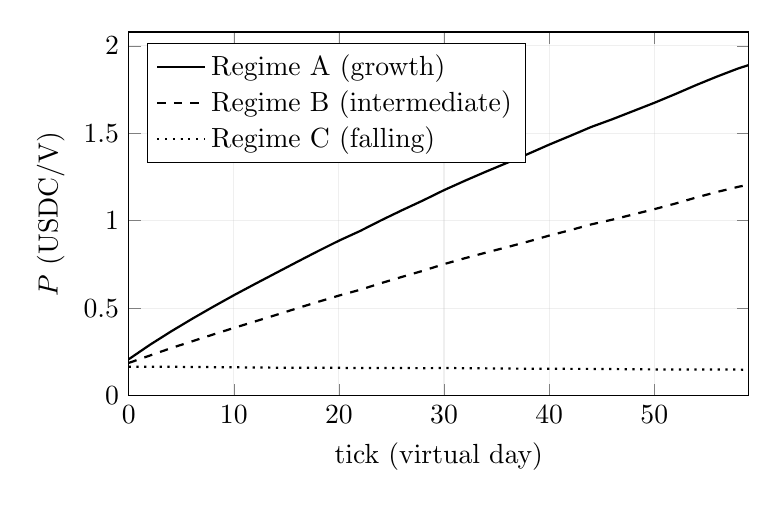
\begin{tikzpicture}
\begin{axis}[
  width=0.78\textwidth, height=6.2cm,
  xlabel={tick (virtual day)}, ylabel={$P$ (USDC/$\V$)},
  legend pos=north west, legend cell align=left,
  grid=major, grid style={opacity=0.25},
  ymin=0, xmin=0, xmax=59,
]
\addplot[thick] coordinates {(0,0.208) (2,0.290) (4,0.366) (6,0.438) (8,0.507) (10,0.574) (12,0.638) (14,0.701) (16,0.764) (18,0.826) (20,0.886) (22,0.941) (24,1.002) (26,1.060) (28,1.116) (30,1.175) (32,1.229) (34,1.281) (36,1.331) (38,1.382) (40,1.435) (42,1.485) (44,1.536) (46,1.580) (48,1.627) (50,1.674) (52,1.724) (54,1.776) (56,1.825) (58,1.871) (59,1.890)};
\addlegendentry{Regime A (growth)}
\addplot[thick, dashed] coordinates {(0,0.187) (2,0.229) (4,0.271) (6,0.310) (8,0.349) (10,0.387) (12,0.424) (14,0.461) (16,0.499) (18,0.536) (20,0.572) (22,0.605) (24,0.643) (26,0.679) (28,0.714) (30,0.752) (32,0.786) (34,0.818) (36,0.849) (38,0.881) (40,0.915) (42,0.946) (44,0.979) (46,1.006) (48,1.036) (50,1.066) (52,1.098) (54,1.133) (56,1.165) (58,1.194) (59,1.206)};
\addlegendentry{Regime B (intermediate)}
\addplot[thick, dotted] coordinates {(0,0.165) (2,0.165) (4,0.165) (6,0.164) (8,0.163) (10,0.162) (12,0.161) (14,0.160) (16,0.160) (18,0.160) (20,0.159) (22,0.158) (24,0.158) (26,0.158) (28,0.157) (30,0.158) (32,0.157) (34,0.156) (36,0.155) (38,0.154) (40,0.154) (42,0.153) (44,0.153) (46,0.152) (48,0.151) (50,0.150) (52,0.150) (54,0.150) (56,0.150) (58,0.149) (59,0.148)};
\addlegendentry{Regime C (falling)}
\end{axis}
\end{tikzpicture}
\caption{Simulator price trajectories for the three regime configurations (seed $23$, $60$ ticks; data from the released \texttt{regime\_analysis} protocol). The growth and falling regimes behave as predicted; the intermediate configuration rises rather than holding flat, reflecting approximate calibration of inflows to emission.}
\label{fig:regimes}
\end{figure}

\paragraph{Long-run price (Proposition~\ref{prop:longrun}).} With $\mu=12$, net emission $e=5000~\V/\text{month}$, investment $\lambda_{\mathrm{inv}}=2000~\text{USDC}/\text{month}$ and initial price $P_0=1$, the limit $g/e=(\lambda_{\mathrm{inv}}+\mu\lambda_{\mathrm{rev}})/e$ maps external-revenue growth directly onto the three regimes (Table~\ref{tab:price}): the stable case reproduces the survival threshold $\lambda_{\mathrm{rev}}=250$ exactly.

\begin{table}[h]
\centering
\begin{tabular}{lrrr}
\toprule
revenue growth $\lambda_{\mathrm{rev}}$ (USDC/mo) & $0$ & $250$ & $500$\\
\midrule
limit $g/e$ (USDC/$\V$) & $0.40$ & $1.00$ & $1.60$\\
regime & C (falling) & B (stable) & A (growth)\\
\bottomrule
\end{tabular}
\caption{Long-run price versus external-revenue growth.}
\label{tab:price}
\end{table}

\paragraph{Fund non-exhaustion (Theorem~\ref{thm:norun}).} With $\rho^*=0.3$ the closed form $F/F_0=(S/S_0)^{1/\rho^*}$ leaves the fund strictly positive at every partial level of exit (Table~\ref{tab:fund}); even a $90\%$ simultaneous exit leaves it nonzero.

\begin{table}[h]
\centering
\begin{tabular}{lrrrrr}
\toprule
Exit & $10\%$ & $30\%$ & $50\%$ & $70\%$ & $90\%$\\
\midrule
$S/S_0$ & $0.90$ & $0.70$ & $0.50$ & $0.30$ & $0.10$\\
$F/F_0$ & $70.4\%$ & $30.5\%$ & $9.9\%$ & $1.8\%$ & $0.05\%$\\
\bottomrule
\end{tabular}
\caption{Fund coverage retained after a simultaneous exit.}
\label{tab:fund}
\end{table}

\paragraph{Unprofitability at scale (Theorem~\ref{thm:fraud}).} With per-transaction audit $a=0.03$, mean size $\bar N=50~\V$ and stake $\Lambda=300~\V$, the audit factor $(1-a)^{W/\bar N}$ alone pushes the expected-profit bound below zero once the theft is large (Table~\ref{tab:fraud}); the lock-up factor $(1-p)^{\tau_{\mathrm{lock}}}$ only lowers it further. Figure~\ref{fig:analytic} plots the fund-retention curve of Theorem~\ref{thm:norun} and the fraud-profit bound $g(W)$ at the default and at the threshold stake.

\begin{table}[h]
\centering
\begin{tabular}{lrrrrr}
\toprule
$W$ ($\V$) & $500$ & $1000$ & $2500$ & $5000$ & $10000$\\
\midrule
wash trades $n$ & $10$ & $20$ & $50$ & $100$ & $200$\\
survive audit $(1-a)^n$ & $73.7\%$ & $54.4\%$ & $21.8\%$ & $4.8\%$ & $0.2\%$\\
$\mathbb{E}[\pi]$ bound ($\V$) & $290$ & $407$ & $311$ & $-48$ & $-277$\\
\bottomrule
\end{tabular}
\caption{Fraud expected-profit bound (audit factor only); it turns negative and tends to $-\Lambda$ as the theft grows.}
\label{tab:fraud}
\end{table}

\begin{figure}[t]
\centering
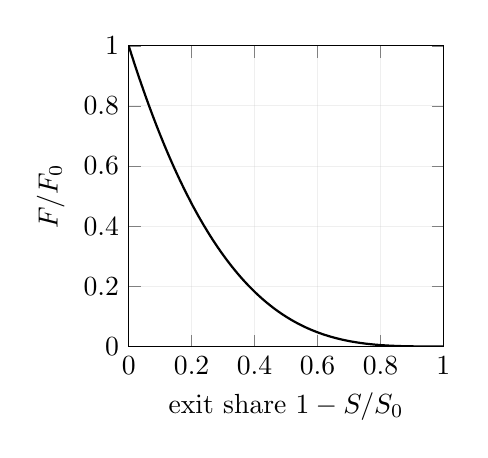
\begin{tikzpicture}
\begin{axis}[
  width=0.46\textwidth, height=5.4cm,
  xlabel={exit share $1-S/S_0$}, ylabel={$F/F_0$},
  domain=0:0.999, samples=200, xmin=0, xmax=1, ymin=0, ymax=1,
  grid=major, grid style={opacity=0.25},
]
\addplot[thick] {(1-x)^(1/0.3)};
\end{axis}
\end{tikzpicture}\hfill
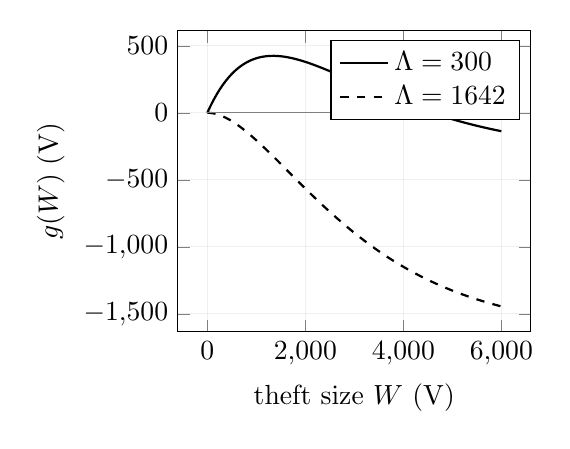
\begin{tikzpicture}
\begin{axis}[
  width=0.5\textwidth, height=5.4cm,
  xlabel={theft size $W$ ($\V$)}, ylabel={$g(W)$ ($\V$)},
  domain=0:6000, samples=300,
  legend pos=north east, legend cell align=left,
  grid=major, grid style={opacity=0.25},
]
\addplot[thick] {exp(-0.00060918*x)*(x+300)-300};
\addlegendentry{$\Lambda=300$}
\addplot[thick, dashed] {exp(-0.00060918*x)*(x+1642)-1642};
\addlegendentry{$\Lambda=1642$}
\addplot[gray, thin, domain=0:6000] {0};
\end{axis}
\end{tikzpicture}
\caption{Left: fund retention under a discounted run, $F/F_0=(S/S_0)^{1/\rho^*}$ with $\rho^*=0.3$ (Theorem~\ref{thm:norun}) --- positive at every partial exit share. Right: the fraud-profit bound $g(W)$ at $c=1$ (Theorem~\ref{thm:deter}); the default stake $\Lambda=300~\V$ leaves a profitable region peaking at ${\approx}{+}425~\V$, while the threshold stake $\Lambda=1642~\V$ makes every theft size loss-making.}
\label{fig:analytic}
\end{figure}

\section{Design guidance}\label{sec:guidance}

The analysis yields a small set of parameter conditions a deployment must satisfy. We collect them here; each is derived above and is a lever the community can tune by governance.

\begin{description}[leftmargin=*,itemsep=3pt]
\item[Bounded inflation.] Keep $K^*\ge\max(1,\varepsilon_{\max})$, so $\Supply/P_{\mathrm{net}}\le\max(1,\varepsilon_{\max})\le K^*$ on the credit-originated supply (Theorem~\ref{thm:stability}; Proposition~\ref{prop:genstab} quantifies the degradation from undetected fraud). A smaller $K^*$ tightens the money-to-value ratio via \eqref{eq:epsilon}. Defaults $K^*=1.5$, $\varepsilon_{\max}=0.95$.
\item[Non-declining price.] Require external-revenue \emph{growth} $\lambda_{\mathrm{rev}}\ge(\mathrm{EmissionRate}\cdot P-\lambda_{\mathrm{inv}})/\mu$; the price then tends to $(\lambda_{\mathrm{inv}}+\mu\lambda_{\mathrm{rev}})/\mathrm{EmissionRate}$ (Propositions~\ref{prop:survival} and~\ref{prop:longrun}). The multiplier $\mu=12$ and the investment inflow are the levers.
\item[Fund solvency under a run.] The discount engages at coverage $\rho<\rho^*$ and keeps $F=F_0(S/S_0)^{1/\rho^*}>0$ for all $S>0$ (Theorem~\ref{thm:norun}); the emission ceiling $\Delta S_{\max}=(F-F_{\min})/P_{\mathrm{target}}$ preserves buy-back capacity. Default $\rho^*=0.3$.
\item[Bounded single-agent exposure.] The credit limit $L(r)=100\,(1+0.5\ln(1+r))$ caps any one member's default loss (I4): at most ${\approx}561~\V$ even at $r=10^4$.
\item[Gated emission.] Mint unbacked $\V$ only when $\confidence(\tau)\ge\theta_{\min}$ (I2). Default $\theta_{\min}=0.6$.
\item[Capital and Sybil resistance.] Vote by $\sqrt{\R}$ with $\R$ soulbound under a dual quorum $\theta$; capital buys no reputation votes, a reputation majority costs $Q/\sqrt{r_0}$ screened, continuously active identities, and the stake quorum must be won separately---capture requires paying both costs (Proposition~\ref{prop:sybil}). Defaults $\theta=0.5$ ($0.66$ for constitutional changes).
\item[Fraud deterrence.] Ensure the per-cluster forfeitable stake $\Lambda\ge\bar N/\ln(1/(1-a))\approx\bar N/a$ (Theorem~\ref{thm:deter}). The levers are the audit rate $a$, the lock-up $\tau_{\mathrm{lock}}$, and required collateral. \emph{The illustrative defaults ($a=0.03$, $\bar N=50$, $\Lambda=300~\V$) fall short of the threshold ($\approx1642~\V$) and must be strengthened.}
\end{description}

Of the illustrative defaults only the fraud-stake condition is unmet; the structural conditions hold by construction, and the price condition is a requirement on realized revenue rather than a parameter choice. Choosing $K^*$, $\mu$, $\rho^*$, $\theta_{\min}$, and the stake/audit parameters within these bounds is the whole of a deployment's economic tuning.

\section{Empirical validation}\label{sec:empirical}

\subsection{Method}

We implemented the full mechanism as a deterministic agent-based simulator with an injected, seeded pseudo-random source, so that a seed reproduces a run bit-for-bit. Stability is graded by five criteria (protocol step V2): (C1) price does not reach zero; (C2) fund coverage $\rho \ge 0.05$ on at least $95\%$ of ticks; (C3) at most $20\%$ of members frozen; (C4) non-negative supply; (C5) invariants clean. We report (C1)--(C4) as \emph{economically stable} separately from (C5), because the (I3) bookkeeping check---the implementation's stricter, confidence-weighted variant of (I3)---has a known drift during the auto-repay/escrow-distribution lifecycle. The protocol comprises: reproduction of reference scenarios (V1); Monte~Carlo over $4$ scenarios $\times\ 30$ seeds (V3); a $192$-point sweep over $(K^*,\mu,\delta^*,\rho^*)$ (V4); combined-attack stress tests (V5); and regime analysis (V6).

\subsection{Results}

Across $315$ runs, no run produced an economic collapse (Table~\ref{tab:results}). The parameter sweep was stable at all $192$ points, indicating the mechanism is not brittle to parameter choice. Combined fraud-plus-bank-run and $70\%$ simultaneous-exit stress tests remained economically stable via the withdrawal queue and escrow burn, and the regime analysis reproduced the predicted ordering of price trajectories (Figure~\ref{fig:regimes}).

\begin{table}[h]
\centering
\begin{tabular}{lrr}
\toprule
Protocol & Runs & Economic collapses\\
\midrule
Monte Carlo (V3) & $120$ & $0$\\
Parameter sweep (V4) & $192$ & $0$\\
Stress tests (V5) & $3$ & $0$\\
\midrule
Total & $315$ & $0$\\
\bottomrule
\end{tabular}
\caption{Validation summary. Full raw outputs accompany the released code.}
\label{tab:results}
\end{table}

\section{Limitations}\label{sec:limitations}

Empirical stability is necessary but not sufficient. Our runs cover $1$--$3$ months of virtual time; slow effects over multi-year horizons are untested. The agents are statistical rather than strategic, so adaptation and political organization by real participants are out of scope; the optimal fraud over independently detected clusters is characterized in Theorem~\ref{thm:deter}, but a fully coordinated adversary (correlating clusters to defeat monitoring) and dynamic timing are not tested empirically. A further strategic gap concerns pricing itself: the auto-score \eqref{eq:autoscore} anchors to the category's rolling price distribution, so a coordinated, gradual drift of declared prices---each step within $|z|\le1$---could shift the reference mean $\mu_c$ over time without ever triggering review. Concentration monitoring and the stochastic audit narrow this channel but the paper does not model such collusive drift. Legal and fiscal questions---jurisdiction, identity/KYC, and the taxation of micro-transactions---lie outside the model. The mechanism therefore constitutes a structurally sound foundation whose behavior with real human participants remains to be established. Section~\ref{sec:extensions} presents design extensions (\emph{Kredo v2}) that address the fraud-stake gap, the collusive-drift channel, the ``grow-or-die'' revenue requirement, and the honest limits of the Sybil argument; each is implemented and verified in the released simulator.

\section{Design extensions (Kredo v2)}\label{sec:extensions}

The audit above surfaced four things worth strengthening: the default fraud stake falls short of the deterrence threshold (Section~\ref{sec:guidance}); the survival condition demands \emph{growth}, not merely a revenue level (Proposition~\ref{prop:survival}); the collusive price drift of Section~\ref{sec:limitations} is unmodeled; and the Sybil argument rests on the per-identity cost rather than the vote rule (Proposition~\ref{prop:sybil}). We describe five extensions that close these gaps. Each is an \emph{opt-in} parameter or service in the released simulator---the default configuration reproduces the results above byte-for-byte---and the four simulator extensions each carry a numerical check from a released experiment. The remaining one, the closed-loop cooperative form, is a legal-and-architectural choice with no simulator toggle.

\subsection{Retention channel and revenue-backed emission}

Proposition~\ref{prop:survival} treats external revenue as an inflow whose \emph{growth} must offset emission. But a fixed share $s$ of realised revenue is retained in the fund each period (the $50/30/15/5$ split of Section~\ref{sec:emission}), which the continuous model omits. Writing $R$ for the trailing revenue \emph{level} and folding retention into $\dot{\mathcal A}=\lambda_{\mathrm{inv}}+sR+\mu\dot{\ExtRev}$, the non-declining-price condition at a constant revenue level ($\dot{\ExtRev}=0$) becomes
\[
R \ \ge\ \frac{e\,P-\lambda_{\mathrm{inv}}}{s},
\]
a \emph{level}, not a growth rate: a steady business sustains the price, converting ``grow or die'' into ``earn steadily.'' A second lever makes the money supply endogenous to earnings---a currency board that caps credit emission at $e(t)\le\eta\,R(t)/P_{\mathrm{target}}$ with the design rule $\eta\le s$; a revenue stop then throttles emission instead of diluting the price. In the simulator, sweeping the constant revenue level walks the economy from falling (at zero revenue) to rising, confirming the level---not its growth---sets the regime. And with the cap active, a mid-run revenue stop starves emission: post-stop supply keeps growing without the cap ($+11.8\mathrm{k}$) but goes slightly negative with it ($-1.6\mathrm{k}$), roughly halving whole-run supply growth ($36.2\mathrm{k}\to17.4\mathrm{k}$) and leaving the price $24\%$ higher.

\subsection{Closed-loop cooperative form}

Two risks the model does not price are legal and arbitrage-theoretic: a freely transferable $\V$ carrying a profit claim resembles a security, and any secondary market in $\V$ would arbitrage against the administered price (I5). Both shrink under a \emph{closed-loop cooperative} reading: $\V$ transfers only between verified members (no external venue, as in the WIR franc), and the activity-weighted dividend is a \emph{patronage refund}---return by participation, not by capital---a long-established cooperative-law construct. With no external venue there is no second price to arbitrage, so (I5) remains the only price by construction. The closedness of the contour is best treated as constitutional, lest ordinary governance re-open it and reintroduce the arbitrage channel. Where an external market is nonetheless wanted, the fund can act as a bounded market-maker quoting a coverage-dependent band around the fundamental price, with its defence capacity published openly (Theorem~\ref{thm:norun}).

\subsection{Sybil defense beyond the vote rule}

Proposition~\ref{prop:sybil} is honest that $\sqrt{\R}$ weighting does not by itself deter splitting. Three additions make the per-identity cost real. \emph{Diversity weighting} sets the vote to $\sqrt{\R}\cdot D$ with $D=\max(d_{\min},1-\mathrm{HHI})$ from the member's counterparty Herfindahl (already computed for anti-fraud): a wash cluster trading within itself has $\mathrm{HHI}\to1$, so $D\to d_{\min}$. \emph{Inactivity decay} $r(t)=r_0\,2^{-\max(0,\Delta t-\text{grace})/T_{1/2}}$ forces every fake to sustain genuine activity or lose its weight. \emph{Vouching with slashing} makes each joiner stake the reputation of $m$ existing vouchers, so an attacker must corrupt real members rather than defeat a KYC provider. In the simulator, at $d_{\min}=0.2$ the diversity weight lifts a reputation-majority attack on a $10^3$-member community from ${\approx}1.4\times10^4$ to ${\approx}6.4\times10^4$ fake identities; decay ($T_{1/2}=180$~d) melts an idle fleet's weight to $56\%$/$28\%$/$7\%$ at $180$/$365$/$730$ days; and at an illustrative reputation price, vouching puts the majority attack near \$$0.78$M.

\subsection{Deterring fraud at the default stake}

Section~\ref{sec:guidance} noted the default stake $\Lambda=300~\V$ is below the threshold $1/\beta\approx1642~\V$. Rather than raise $\Lambda$ punitively, make the lock-up grow with the amount, $\tau_{\mathrm{lock}}(W)=\tau_0+wW$, which steepens the survival decay of Theorem~\ref{thm:deter}.

\begin{corollary}[Deterrence at the default stake via vesting]\label{cor:vesting}
Under the amount-scaled lock-up $\tau_{\mathrm{lock}}(W)=\tau_0+wW$, the survival probability becomes $q(W)=c_0\,e^{-\beta' W}$ with $\beta'=\beta+w\,\ln\!\bigl(1/(1-p)\bigr)$ and $c_0=(1-p)^{\tau_0}$. Hence the deterrence threshold $\Lambda\ge1/\beta'$ is met for a fixed $\Lambda$ by any
\[
w\ \ge\ \frac{1/\Lambda-\beta}{\ln\!\bigl(1/(1-p)\bigr)} .
\]
\end{corollary}
\begin{proof}
Each of the $\tau_0+wW$ lock-up periods survives detection with probability $1-p$, contributing $(1-p)^{\tau_0+wW}=c_0\,e^{-wW\ln(1/(1-p))}$; multiplying by the audit factor $(1-a)^{W/\bar N}=e^{-\beta W}$ gives $q(W)=c_0e^{-\beta'W}$ with the stated $\beta'$. Replacing $\beta$ by $\beta'$ in Theorem~\ref{thm:deter}, $\Lambda\ge1/\beta'$ forces $W^\dagger\le0$; solving $\beta+w\ln(1/(1-p))\ge1/\Lambda$ for $w$ gives the bound.
\end{proof}

With a per-day cluster-detection probability $p=0.05$ acting over the amount-scaled vesting (the base lock-up held non-detecting, matching the conservative audit-only baseline), the bound gives $w\approx0.053$ days per V---about $5.3$ days of extra vesting per $100~\V$. The simulator's \texttt{FraudDeterrenceService} then drives the optimum down through the profitable baseline: $+425\to+67\to0~\V$ at $w=0,\,0.02,\,0.053$, so the fraud is non-positive (deterred) at the unchanged $\Lambda=300~\V$. Escalating a flagged cluster's audit to $a=0.30$ is even sharper, giving $1/\beta\approx140~\V<\Lambda$ outright.

\subsection{A collusive-drift detector}

The collusive drift of Section~\ref{sec:limitations} is caught by comparing the category's short ($T_s$) and long ($T_l$) price windows: a linear drift $v$ holds their medians a steady $v(T_l-T_s)/2$ apart, so flagging $|\mu_s-\mu_l|>\kappa\sigma$ bounds the sustainable undetected drift to
\[
v^\ast=\frac{\kappa\sigma}{(T_l-T_s)/2}\ \bigl(=\kappa\sigma/137.5\ \text{at }T_l/T_s=365/90\bigr).
\]
The variance $\sigma$ must be estimated on \emph{detrended} prices (first differences), or a large drift inflates the threshold and hides itself; a CUSUM chart complements the windowed rule by catching small-step drift. In the simulator ($\kappa=1.5$, $\sigma=10$), $v^\ast\approx0.11~\V$/day: a drift at half $v^\ast$ escapes the window rule but takes ${\approx}5$ years to double a price---economically pointless while the cluster stays exposed to concentration monitoring---and a drift at twice $v^\ast$ is flagged; the CUSUM catches the slow drift the window smooths over.

\section{Conclusion}

Kredo demonstrates that a coherent ethical stance---reward for creation, symmetry of fate, transparency, and power from contribution---can be compiled into a precise mechanism whose intended properties are provable and machine-checkable. The compensatory-emission coefficient bounds inflation under defaults, fund operations are price-neutral and the fund survives any partial run, governance capture requires winning both the reputation and the stake quorum, large frauds are strictly loss-making and beyond the derived stake threshold even the optimal adaptive fraud is unprofitable, and a minimal external-revenue-growth condition governs survival. A deterministic simulator corroborates structural resilience across $315$ runs. The open release invites replication, adversarial analysis, and extension toward a small live deployment.

\section*{Data and code availability}

The mechanism specification, full derivations, the simulator, the experiment protocols, and the raw results are openly available at \url{https://github.com/fedorello/kredo-model} under the MIT license. The v2 design extensions of Section~\ref{sec:extensions} are documented under \texttt{improvements/} and verified by the \texttt{retention\_analysis}, \texttt{sybil\_attack}, \texttt{fraud\_deterrence}, and \texttt{collusive\_drift} experiments.

\begin{thebibliography}{99}
\bibitem{gesell1916} S.~Gesell. \emph{The Natural Economic Order}. Self-published, 1916 (English translation, Peter Owen, 1958).
\bibitem{greco2009} T.~H.~Greco. \emph{The End of Money and the Future of Civilization}. Chelsea Green, 2009.
\bibitem{stodder2009} J.~Stodder. Complementary credit networks and macroeconomic stability: Switzerland's Wirtschaftsring. \emph{Journal of Economic Behavior \& Organization}, 72(1):79--95, 2009.
\bibitem{circles2020} Circles~UBI. \emph{Circles: A Basic Income Money System} (whitepaper). 2020.
\bibitem{gooddollar2021} GoodDollar. \emph{GoodDollar: A Distributed Basic Income} (whitepaper), v2. 2021.
\bibitem{nakamoto2008} S.~Nakamoto. \emph{Bitcoin: A Peer-to-Peer Electronic Cash System}. 2008.
\bibitem{lalley2018} S.~P.~Lalley and E.~G.~Weyl. Quadratic voting: how mechanism design can radicalize democracy. \emph{AEA Papers and Proceedings}, 108:33--37, 2018.
\bibitem{buterin2019} V.~Buterin, Z.~Hitzig, and E.~G.~Weyl. A flexible design for funding public goods. \emph{Management Science}, 65(11), 2019.
\bibitem{douceur2002} J.~R.~Douceur. The Sybil attack. In \emph{Proc.\ IPTPS}, LNCS 2429, pp.~251--260, 2002.
\bibitem{bonabeau2002} E.~Bonabeau. Agent-based modeling: methods and techniques for simulating human systems. \emph{PNAS}, 99(suppl.~3):7280--7287, 2002.
\end{thebibliography}

\end{document}
